% !TeX root=../main.tex 
\section{Результати роботи програми}
\label{sec:result_analyse}
\jointitles
\subsection{Результати підрахунку констант}
Для формули \eqref{eq:model_final} було чисельно пораховано коефіцієнт $C_{p}$, для кожного $p$ від 0 до 0.9 з кроком 0.1. Результати наведені на~\imref{fig:integ_cp}.

\begin{figure}[H]
    \centering
    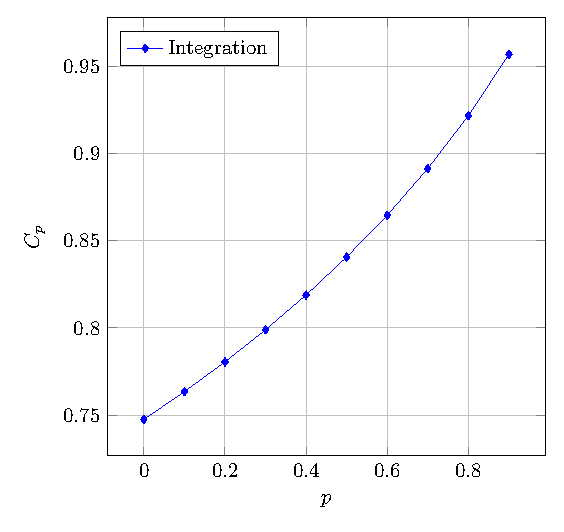
\includegraphics[scale=0.8]{chapter_Practice/img/integ_cp}
    \caption{Значення $C_{p}$, отримані методом чисельного інтегрування}
    \label{fig:integ_cp}
\end{figure}

\subsection{Результати роботи моделера}

Для формули \eqref{eq:model_final} було промодельовано поведінку водіїв на парковці довжини $x=100000$ і емпірично визначено коефіцієнт $C_{p}$, для кожного $p$ від 0 до 0.9 з кроком 0.1. Результати наведені на ~\imref{fig:simul_cp}.

\begin{figure}[H]
    \centering
    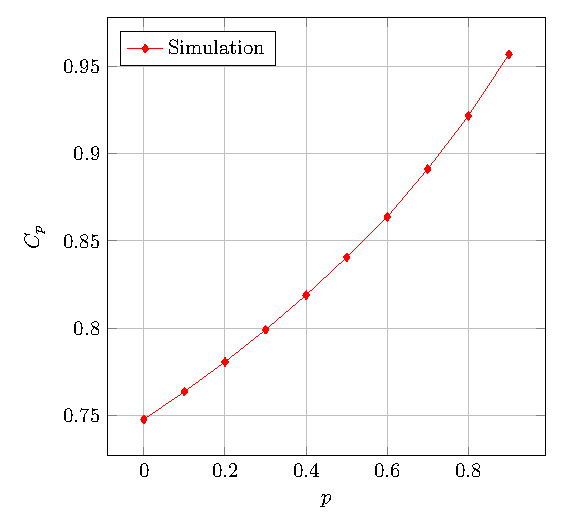
\includegraphics[scale=0.8]{chapter_Practice/img/simul_cp}
    \caption{Значення $C_{p}$, отримані методом імітаційного моделювання}
    \label{fig:simul_cp}
\end{figure}

З \imref{fig:composite_cp} нескладно помітити, що теоретичний результат майже співпав з результатом моделювання:
\begin{figure}[H]
    \centering
    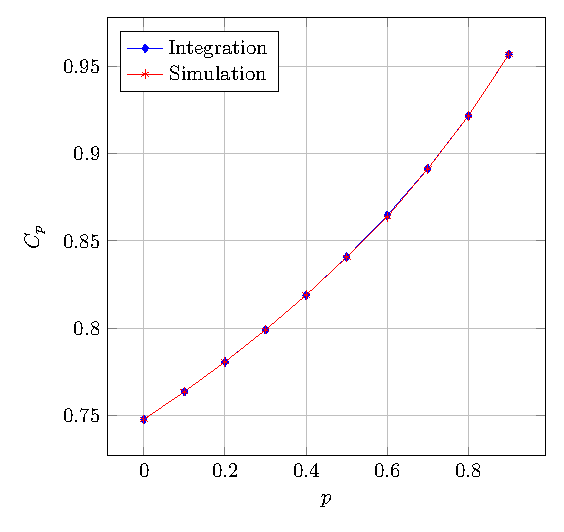
\includegraphics[scale=0.8]{chapter_Practice/img/composite_cp}
    \caption{Порівняння значень $C_{p}$, отриманих різними методами}
    \label{fig:composite_cp}
\end{figure}

Для двовимірного випадку існує припущення, так звана гіпотеза Паласті, що відношення середньої кількості автомобілів до загальної площі парковки прямує до $C^2 \approx 0.56$, але це не доведений факт \cite{MathWorldRenyi}. Було проведено експеримент на розмірах 50x50, 100x100, 200x200, і результати вийшли відповідно 0.7, 0.6 та 0.58, тобто ймовірно, що припущення правдиве, але для перевірки на дуже великих розмірах парковки необхідні дуже потужні обчислювальні ресурси через велику складність двовимірного алгоритму.
